\problemname{Wordfeud}
Wordfeud är ett scrabble/alfapet-liknande spel där man ska lägga ut bokstavsbrickor på en rutig spelplan så att det bildas ord. Orden kan läggas antingen från vänster till höger eller uppifrån och ned. Varje bokstav ger en viss poäng. Dessutom finns ett antal specialrutor på spelplanen, som kan vara av fyra typer:

\begin{itemize}
	\item \texttt{DL} (double letter): bokstavspoängen för en bricka på denna ruta dubbleras
	\item \texttt{TL} (triple letter): bokstavspoängen för en bricka på denna ruta tredubblas
	\item \texttt{DW} (double word): poängen för hela ordet dubbleras om rutan täcks
	\item \texttt{TW} (triple word): poängen för hela ordet tredubblas om rutan täcks
\end{itemize}

När man räknar ut poängen för ett ord börjar man med att summera bokstavspoängen, med eventuell multiplikation på varje bokstav. När summan är uträknad multipliceras den med eventuella ordmultiplikatorer. Observera att om ordet ligger på flera \texttt{DW}- eller \texttt{TW}-rutor kan poängen multipliceras flera gånger.

I den här uppgiften tänker vi oss en tom $10$x$10$ spelplan där raderna och kolumnerna är numrerade enligt figuren. Skriv ett program som, givet specialrutornas placering på spelplanen och det ord du tänker lägga ut, beräknar den högsta poäng du kan få om du får lägga ordet var du vill (men hela ordet inom spelplanen).

\begin{figure}[!h]
	\centering
	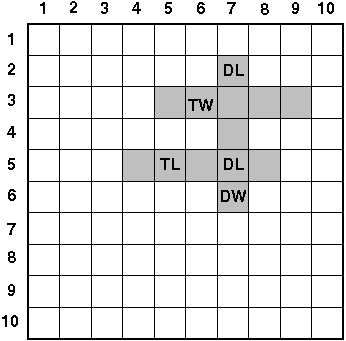
\includegraphics[width=0.35\textwidth]{wordfeud}
	\caption{Spelplanen i exemplet med specialrutorna utmärkta. De skuggade områdena visar tre exempel på placering av “ordet” $56141$. Den lodräta placeringen ger $2\cdot(2\cdot5+6+1+2\cdot4+1)=52$ poäng, den vågräta på rad $3$ ger $51$ poäng och den vågräta på rad $5$ ger $33$ poäng.}
\end{figure}

\section*{Input}
Den första raden innehåller $N$ ($1\leq N \leq 10$), antalet specialrutor.

De följande $N$ raderna beskriver vardera en specialruta. Varje ruta består av två tal, raden respektive
kolumnen för specialrutan (båda i intervallet $1$ till $10$), samt specialrutans typ (\texttt{DL}, \texttt{TL}, \texttt{DW} eller \texttt{TW}).

Slutligen följer en sista rad, innehållandes ordet som ska läggas. För enkelhetens skull har varje bokstav redan ersatts med sitt poängvärde, en siffra mellan $0$ och $8$. Ordet kan ha upp till $7$ bokstäver.

\section*{Output}
Skriv ut ett heltal: den maximala poängen som är möjlig att få för det givna ordet.

\section*{Poängsättning}
Din lösning kommer att testas på en mängd testfallsgrupper.
För att få poäng för en grupp så måste du klara alla testfall i gruppen.

\noindent
\begin{tabular}{| l | l | p{12cm} |}
  \hline
  \textbf{Grupp} & \textbf{Poäng} & \textbf{Gränser} \\ \hline
  $1$    & $50$          & \texttt{DW} och \texttt{TL} förekommer inte i indatan.  \\ \hline
  $2$    & $50$          & Inga ytterligare begränsningar.  \\ \hline
\end{tabular}
